\documentclass{oxmathproblems}
\usepackage{graphicx}
\usepackage{hyperref}
\usepackage{footmisc}
\usepackage{listings}
\graphicspath{{imagenes/}} 

\course{EE447 Mobile Internet HW 1: The Optimal Connectivity Determination in Uncertain Graphs}

\newtheorem{theorem}{Theorem}
\newtheorem{lemma}[theorem]{Lemma}
\newtheorem{proposition}[theorem]{Proposition}
\newtheorem{corollary}[theorem]{Corollary}
\newtheorem{exercise}{Exercise}
\newtheorem{definition}{Definition}
\theoremstyle{definition}
\lstset{
	keywordstyle=\color{blue!70}\bfseries, %设置关键词为蓝色,需要引xcolor宏包
	basicstyle=\ttfamily, 
	commentstyle=\ttfamily, %基本和注释的字体都使用默认的等宽,而非texlive调用的中文字体
	showstringspaces=false, %不显示中间的空格
	frame=shadowbox,
	rulesepcolor=\color{red!20!green!20!blue!20},
}
\makeatletter \renewenvironment{proof}[1][Proof] {\par\pushQED{\qed}\normalfont\topsep6\p@\@plus6\p@\relax\trivlist\item[\hskip\labelsep\bfseries#1\@addpunct{.}]\ignorespaces}{\popQED\endtrivlist\@endpefalse} \makeatother
\makeatletter
\renewenvironment{solution}[1][Solution] {\par\pushQED{\qed}\normalfont\topsep6\p@\@plus6\p@\relax\trivlist\item[\hskip\labelsep\bfseries#1\@addpunct{.}]\ignorespaces}{\popQED\endtrivlist\@endpefalse} \makeatother

\begin{document}
\begin{center}
	% Please write down your name, student id and email.
	Name: Hongjie Fang \quad Student ID:518030910150 \quad Email: \href{mailto:galaxies@sjtu.edu.cn}{galaxies@sjtu.edu.cn}
\end{center}
Determining the source-destination connectivity in uncertain graphs has wide applications in real life, e.g., routing detection, information diffusion control, etc. For an uncertain graph, each edge exists independently with some probability, and the existence of each edge can be unraveled through edge testing with a certain cost. Our goal is to determine whether source s and destination t are connected or not with the minimum expected cost.
	
Given the following several kinds of uncertain graphs, please provide the corresponding optimal strategy with the minimum expected cost, and prove its optimality, respectively.
\begin{enumerate}
\item For the pyramid graph in Figure \ref{fig1}, each edge exists with probability $p$, and the cost of testing the existence of each edge is $1$. 
\begin{figure}[htbp]
\label{fig1}
\centering
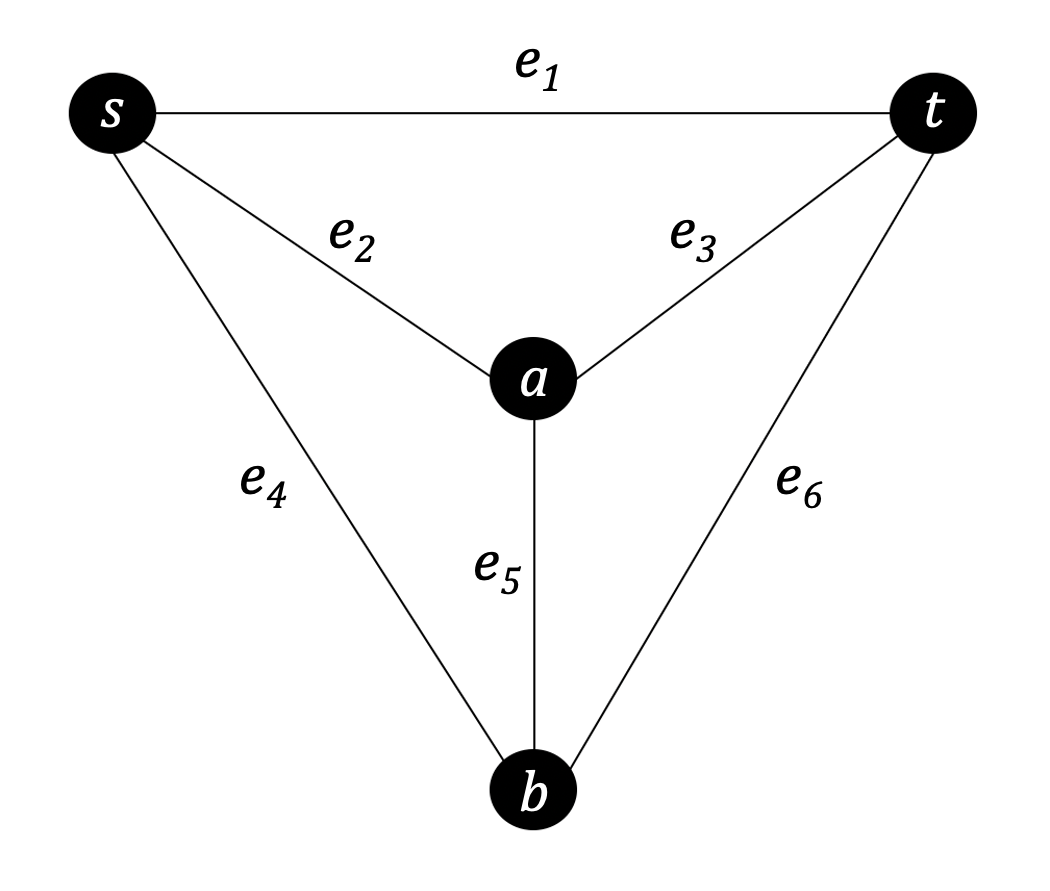
\includegraphics[width=5.5cm]{1.png}
\caption{Pyramid Graph}
\end{figure}
\begin{solution}
	We number the vertices and edges for convenience of explanations, as Figure \ref{fig1} shown. Then we make the following clarifications.
	\vspace{-0.2cm}
	\begin{enumerate}
		\item To prove $s$ is connected with $t$, we only need to find one available path.
		\item To prove $s$ is disconnected with $t$, every possible path between $s$ and $t$ should be unavailable. Specially, in the pyramid graph, every edge may contribute to the connectivity between $s$ and $t$, so every edge should be checked to determine that every path between $s$ and $t$ is unavailable, \textit{i.e.}, $s$ is disconnected with $t$.
	\end{enumerate}
	\vspace{-0.2cm}

	There are totally 5 paths between $s$ and $t$, listed in Table \ref{tab1}.
	
	\vspace{-0.1cm}
	\begin{table}[htbp]\label{tab1}
		\centering
		\caption{The paths between $s$ and $t$ and their probabilities}
		\begin{tabular}{|c|c|c|c|c|c|}
			\hline
			\textbf{Path Number} & $P_1$ & $P_2$ & $P_3$ & $P_4$ & $P_5$ \\ \hline 
			\textbf{Path} & $s\stackrel{e_1}{\rightarrow}t$ & $s\stackrel{e_2}{\rightarrow}a\stackrel{e_3}{\rightarrow}t$ & $s\stackrel{e_4}{\rightarrow}b\stackrel{e_6}{\rightarrow}t$ & $s\stackrel{e_2}{\rightarrow}a\stackrel{e_5}{\rightarrow}b\stackrel{e_6}{\rightarrow}t$ & $s\stackrel{e_4}{\rightarrow}b\stackrel{e_5}{\rightarrow}a\stackrel{e_3}{\rightarrow}t$ \\ \hline
		\end{tabular}
	\end{table}

	\iffalse
	Define $E(C \mid E_e \subseteq E, E_n \subseteq E, E_e \cap E_n = \varnothing)$ as the minimum expected cost to determine the connectivity between $s$ and $t$ under the condition that edges in $E_e$ exist, edges in $E_n$ don't exist, and other edges are undetermined. Here $E = \{e_i \mid i=1,2,3,4,5,6\}$ denotes the edge set in the pyramid graph, and $C$ represents ``connectivity''.
	
	Then, we can derive the formula of $E(C\mid E_e, E_n)$ as follows.
	
	$$
	E(C\mid E_e, E_n)=\left\{\begin{aligned}
	& 0, &&&& D(E_e, E_n) = 1 \\
	& 1 + \min_{e \in E \backslash E_e \backslash E_n}\{&&p\cdot E(C\mid E_e \cup \{e\}, E_n) && \\
	&&& + (1-p)\cdot E(C\mid E_e, E_n \cup \{e\})\}, && D(E_e, E_n) = 0
	\end{aligned}
	\right.
	$$
	
	where
	
	$$
	D(E_e, E_n) = \left\{\begin{aligned}
	& 1, \quad && \textrm{current $E_e$ and $E_n$ conditions are able to} \\
	&&& \textrm{determine the connectivity between $s$ and $t$} \\
	& 0, \quad && \textrm{current $E_e$ and $E_n$ conditions arew not able to} \\
	&&& \textrm{determine the connectivity between $s$ and $t$} \\
	\end{aligned}\right.
	$$
	
	\textit{e.g.}, $D(\{e_1\}, \varnothing) = 1$ and $D(\{e_2, e_4\},\{e_3\}) = 0$.
	
	Then, our strategy is as follows.
	
	\begin{enumerate}
		\item [\textbf{Step 1}. ] Calculate $E(C\mid E_e, E_n)$ for every possible $E_e, E_n$. Actually it can be done by calculating $E(C\mid \varnothing, \varnothing)$, which is the minimum expected cost of the graph. 
		\item [\textbf{Step 2}. ] Let $E_e = \varnothing$ and $E_n = \varnothing$.
		\item [\textbf{Step 3}. ] If we are able to determine the connectivity between $s$ and $t$ under the condition that edges in $E_e$ exist and edges in $E_n$ don't exist, then output the result and finish the process; otherwise, go to Step 4.
		\item [\textbf{Step 4}. ] Check the edge $e$ which can minimize the expected cost, that is,	
		$$
		e = \arg\min_{e \in E\backslash E_e\backslash E_n} \{p\cdot E(C\mid E_e \cup \{e\}, E_n) + (1-p)\cdot E(C\mid E_e, E_n \cup \{e\})\}
		$$
		 
		If edge $e$ exists, then let $E_e = E_e \cup \{e\}$; otherwise, let $E_n = E_n \cup \{e\}$. Then, go to Step 3.
	\end{enumerate} 
	
	\textbf{Optimality Explanation}. Actually, this algorithm considers every possibilities, and calculate the minimum expected cost under certain conditions from the beginning to the end. Therefore, the strategy should be optimal and the minimum expected cost is $E(C\mid \varnothing, \varnothing)$.
	\fi
	
	According to the optimal policy which is introduced in the class \footnote{\label{fu2014}Luoyi Fu, Xinbing Wang, and P. R. Kumar. ``Optimal determination of source-destination connectivity in random graphs.'' \textit{Proceedings of the 15th ACM international symposium on Mobile ad hoc networking and computing}. 2014.}, obeying the following rules makes the strategy optimal.
	
	\begin{enumerate}
		\item[\textbf{Rule 1}. ] Test if direct edge exists between $s$ and $t$;
		\item[\textbf{Rule 2}. ] List all paths connecting $s$ and $t$ with the minimum number of potential edges, and find the set $M$ that contains the minimum potential cut between $s$ and $t$.
		\item[\textbf{Rule 3}. ] Sharpen Rule 2 by specifying which particular edge in $M$ should be tested, \textit{i.e.}, test any edges in $M$ connecting $s$ and $t$.
	\end{enumerate}

	To apply those rules in this situation, we can derive the strategy shown in Figure \ref{fig2}.
	\begin{figure}[htbp]
		\centering
		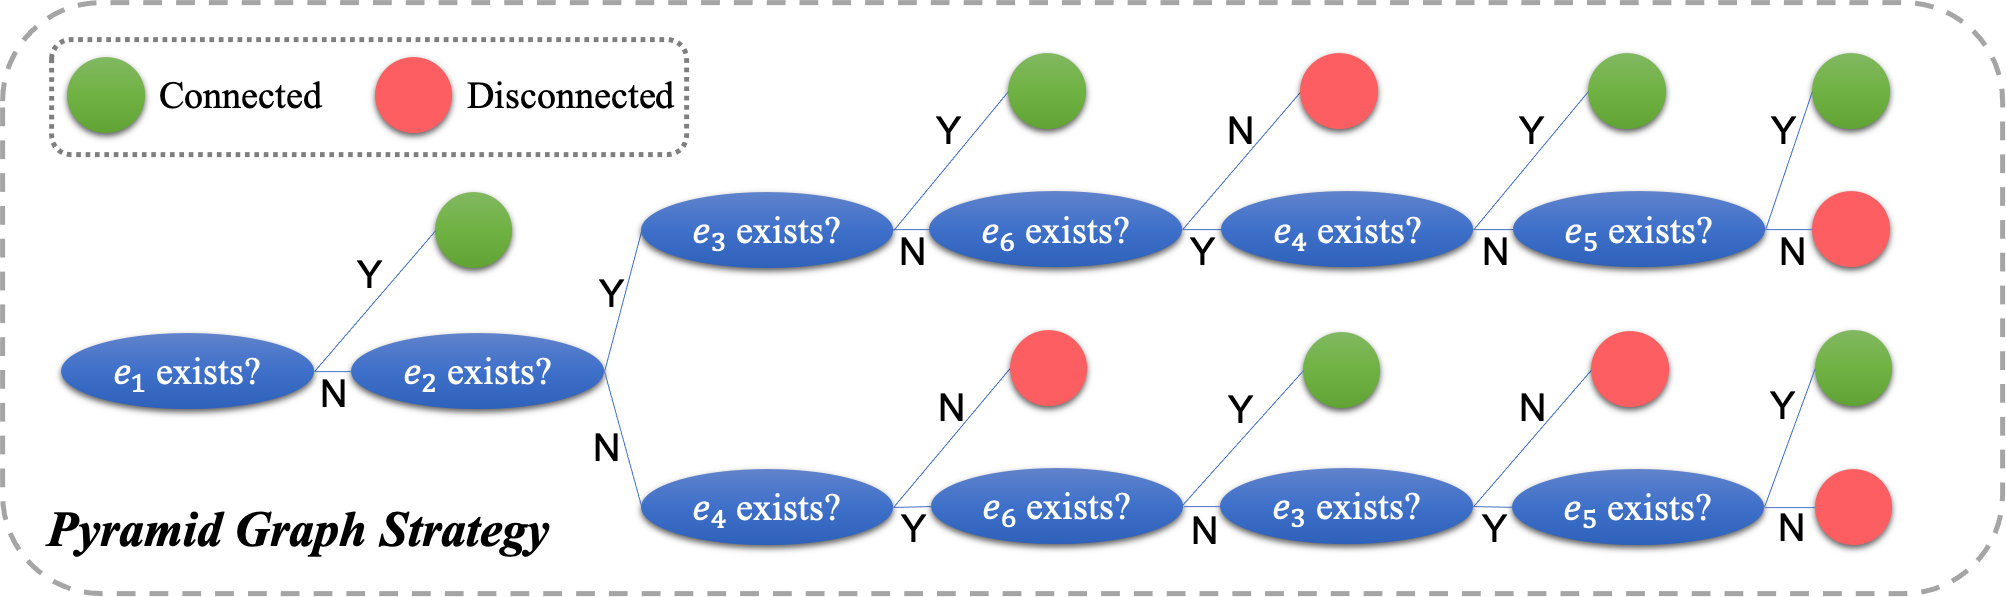
\includegraphics[width=15cm]{1-strategy.png}
		\caption{The Strategy for Pyramid Graph}
		\label{fig2}
	\end{figure}
	
	\textbf{Optimality Explanation}. Our strategy obey the previous rules, according to the theorem of the paper\footref{fu2014}, our strategy is optimal with minimum expected cost as follows.
	$$
	E = p + 3(1-p)p^2 + 3(1-p)^3 + 4(1-p)^3p + 4(1-p)^2p^2 + 5(1-p)^2p^3 + 10(1-p)^3p^2  + 5(1-p)^4p
	$$
\end{solution}
\clearpage
\item For the graph with $m$ parallel edges between nodes $s$ and $t$, edges are labeled $e_1$ through $e_m$ as shown in Figure \ref{fig3}. The probability that edge $e_i$ $(i=1,2,\cdots,m)$ exists is $p_i$. And the test cost of edge $e_i$ is $t_i$. 
\begin{figure}[htbp]
	\centering
	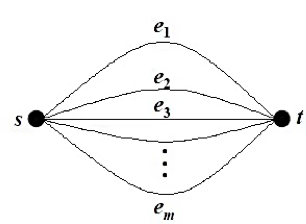
\includegraphics[width=5cm]{2.png}
	\caption{Parallel Graph}
	\label{fig3}
\end{figure}
\begin{solution}
	We make the following clarifications.
	\vspace{-0.2cm}
	\begin{enumerate}
		\item To prove $s$ is connected with $t$ in the parallel graph, we only need to find one available edge of the parallel graph.
		\item To prove $s$ is disconnected with $t$ in the parallel graph, every edge of the parallel graph should be checked.
	\end{enumerate}
	Let us define the \textbf{revenue} $r_i$ of edge $e_i$ to be $p_i / t_i$, which indicates that the average percentage of determined connectivity per unit of cost if we check the $i$-th edge. We present our strategy as follows. {\color{blue} Intuitively, we can just sort the edges by their revenue $r_i$ in a descending order, and check them one by one.} 
	
	Now, let us prove the strategy gives optimal solution with minimum expected cost.
	\begin{definition}[Static strategy]\label{def1} A \textbf{static strategy} means that we won't change the checking order when new information is collected. Let $t_i$ denotes the order that edge $e_i$ is checked in a strategy. Then, a static strategy can be represented as $\{t_1, t_2, \cdots, t_m\}$.
	\end{definition}
	\begin{definition}[Dynamic strategy]\label{def2} A \textbf{dynamic strategy} means that we may change the checking order when new information is collected.
	\end{definition}

\begin{figure}[htbp]
	\centering
	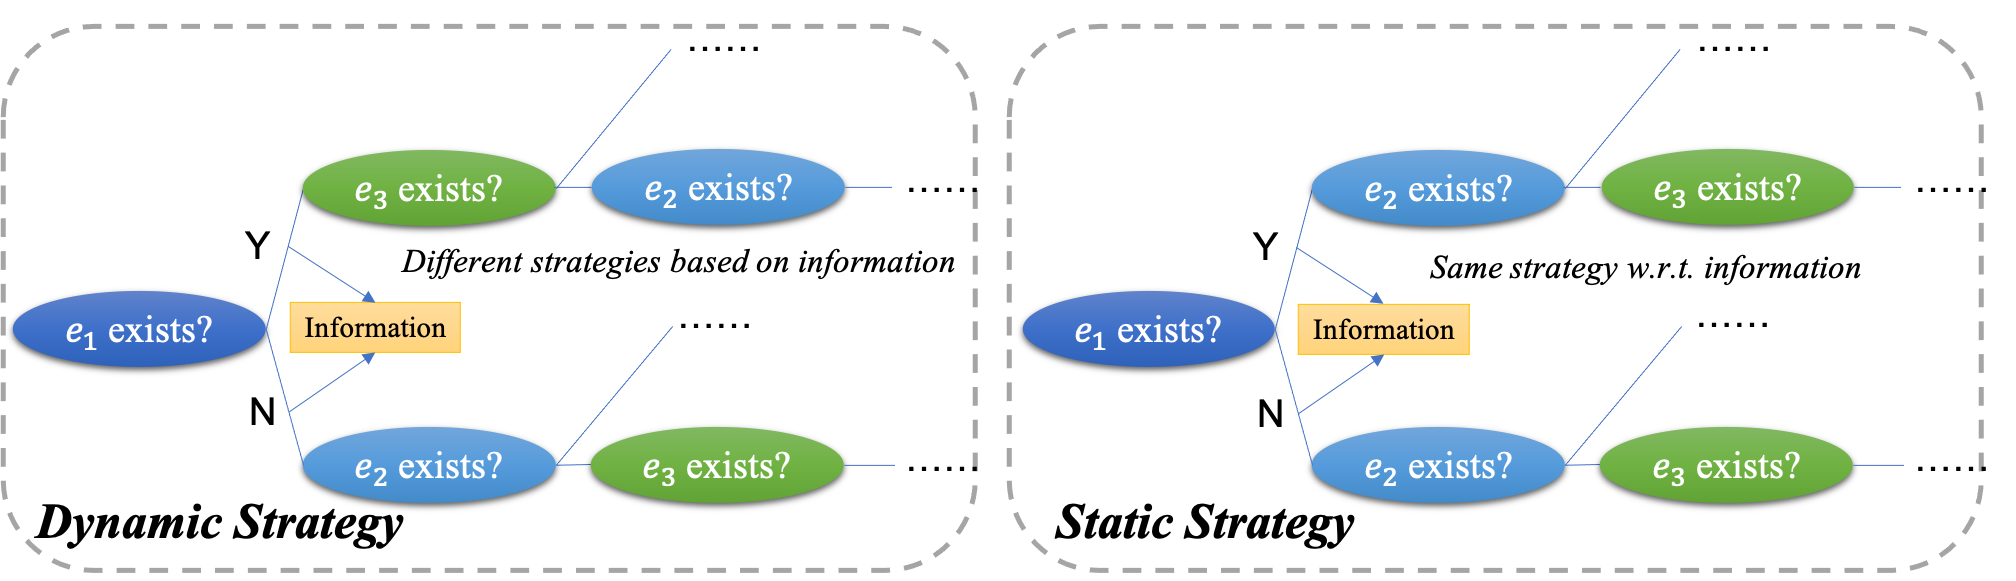
\includegraphics[width=12cm]{2-dynamic-static.png}
	\caption{Dynamic Strategy and Static Strategy}
	\label{fig4}
\end{figure}
	
	\begin{lemma}\label{lemma1}
	In parallel graph, there is always a static strategy that is not worse than a given dynamic strategy.
	\end{lemma}
	\begin{proof}
	According to the clarifications, if our new-collected information is that an edge exists, then the whole process is finished, we don't need to change the following order. If the new-collected information is that an edge does not exist, then we can direct apply the order of dynamic strategy without waiting for the collected ``information'' and get a static strategy with the same quality. Hence, we can always transform a dynamic strategy to a static strategy that is not worse than dynamic one.
	\end{proof}
	\begin{lemma}\label{lemma2}
		Our strategy is a static strategy.
	\end{lemma}
	\begin{proof}
	We won't change the checking order during the checking process, hence our strategy is a static strategy.
	\end{proof}
	Lemma \ref{lemma1} indicates that we only need to focus on the statis strategies, since dynamic strategies can always be replaced with static strategies. Therefore, in the following discussions, the word ``strategy'' stands for static strategy by default.
	\begin{definition}[Ordered pair]\label{def3}
	Given a strategy, if edge $e_i$ is checked before edge $e_j$ in the strategy and the revenue of $e_i$ is less than the revenue of $e_j$, \textit{i.e.}, $t_i < t_j$ and $r_i < r_j$, then $(e_i, e_j)$ is an \textbf{ordered pair}.
	\end{definition}
	\begin{lemma}\label{lemma3}
		Our strategy has no ordered pair.
	\end{lemma}
	\begin{proof}
	Since we sort the edges by their revenue $r_i$ in a descending order and check them according to this order, no ordered pair will be produced in this process.
	\end{proof}
	\begin{definition}[Consecutive ordered pair]\label{def4} Given a strategy, an ordered pair $(e_i, e_j)$ of the strategy is a \textbf{consecutive ordered pair} if and only if $t_i + 1 = t_j$.
	\end{definition}
	\begin{lemma}\label{lemma4}
		Any strategy that has an ordered pair must have a consecutive ordered pair.
	\end{lemma}
	\begin{proof}
		Assume $(e_i, e_j)$ is an ordered pair, \textit{i.e.}, $r_i < r_j$. then $(e_i, e_{i+1}), \cdots, (e_{j-1}, e_j)$ must contain at least one consecutive pair; otherwise, $r_i \ge r_{i+1} \ge \cdots \ge r_j$ will derive a contradiction with the fact that $r_i < r_j$.
	\end{proof}
	
	\begin{lemma}\label{lemma5}
		Given a strategy with consecutive ordered pairs, we can swap the edge order of a consecutive ordered pair and get a better strategy. In other words, if a strategy $\{t_1, t_2, \cdots, t_{i-1}, t_i, t_{i+1}, \cdots, t_{j-1}, t_j, t_{j+1}, \cdots, t_m\}$ has a consecutive ordered pair $(e_i, e_j)$, then strategy $\{t_1, t_2, \cdots, t_{i-1}, t_j, t_{i+1}, \cdots, t_{j-1}, t_i, t_{j+1}, \cdots, t_m\}$ is better than the original strategy.
	\end{lemma}
	\begin{proof}
		The expected cost of the original strategy and the new strategy are as follows:
		$$
		\begin{aligned}
		E_o &= \cdots(t_i + (1-p_i)(t_j + (1-p_j)(\cdots))) \\
		E_n &= \cdots(t_j + (1-p_j)(t_i + (1-p_i)(\cdots)))
		\end{aligned}
		$$
		
		Hence,
		$$
		E_n - E_o = t_j + (1-p_j)t_i - t_i- (1-p_i)t_j = p_it_j-p_jt_i
		$$
		
		Notice that, since $(e_i, e_j)$ is a consecutive ordered pair, then $r_i < r_j$, \textit{i.e.}, $p_i/t_i < p_j/t_j$. Since $t_i, t_j > 0$, we have $E_n - E_o = p_it_j - p_jt_i < 0$, \textit{i.e.} $E_n < E_o$. Therefore, our new strategy is better than the original strategy in the aspect of expected cost. 
	\end{proof}
	\begin{theorem}\label{th6}
	The strategy with no ordered pair is the optimal strategy with lowest expected cost.
	\end{theorem}
	\begin{proof}
		Suppose another strategy with at least one ordered pair is optimal, \textit{i.e.}, better than the strategy with no ordered pair. Then according to Lemma \ref{lemma4}, the strategy must include at least one consecutive ordered pair. Then from Lemma \ref{lemma5} we know that, swapping the consecutive ordered pair can form a better strategy, which contradicts with the optimality of the strategy. Hence, the strategy with no ordered pair is the optimal strategy with lowest expected cost.
	\end{proof}
	\begin{theorem}\label{th7}
		Our strategy is the optimal strategy with lowest expected cost.
	\end{theorem}
	\begin{proof}
		From Lemma \ref{lemma3}, our strategy has no ordered pair. According to Theorem \ref{th6}, the strategy with no ordered pair is the optimal strategy with lowest expected cost. Then, our strategy is the optimal strategy with lowest expected cost.
	\end{proof}

	Theorem \ref{th7} shows that our strategy is the optimal strategy with lowest expected cost.
\end{solution}
\clearpage

\item  \textbf{(Optional, with additional bonus up to 2\% of your final course score.)} For the series-parallel graph consisting of $n$ parallel graph labeled $P^1_{m_1}, \cdots, P^n_{m_n}$, arranged in series. Let the $i$-th edge in the $j$-th parallel graph be represented as $e_{ij}$ $(1\leq j \leq n, 1\leq i\leq m_j)$. Edge $e_{ij}$ exists with probability $p_{ij}$ and has test cost $c_{ij}$. 
\begin{figure}[htbp]
\centering
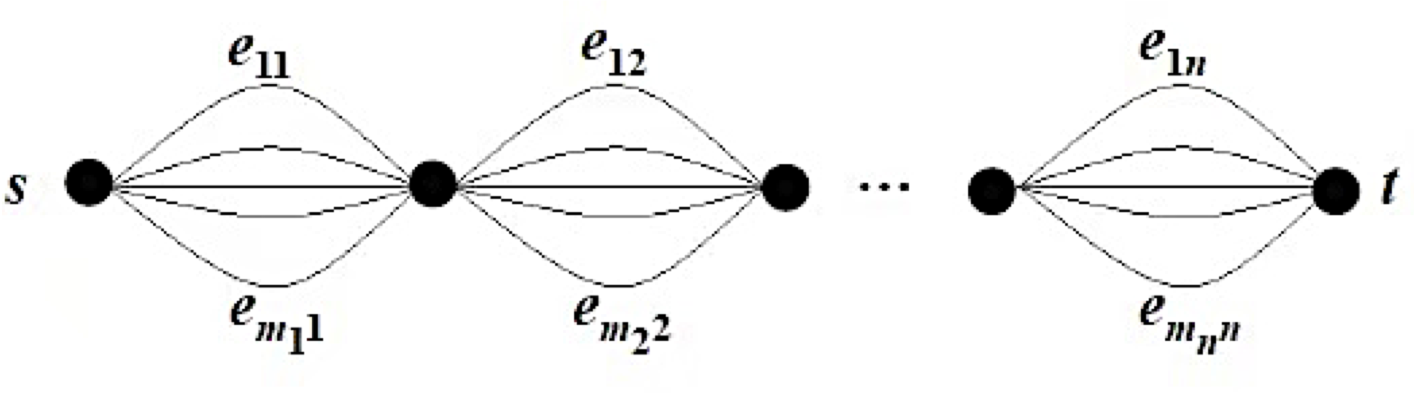
\includegraphics[width=11cm]{3.png}
\caption{Series-Parallel Graph}
\label{fig5}
\end{figure}
\begin{solution}We make the following clarifications.
	\vspace{-0.2cm}
	\begin{enumerate}
		\item To prove $s$ is connected with $t$ in the series-parallel graph, every parallel graph should be connected.
		\item To prove $s$ is disconnected with $t$ in the parallel graph, at least one parallel graph should be disconnected.
	\end{enumerate}

	The series-parallel graph consists of several parallel graph, then according to the proof in Problem 2, we propose the following lemma.
	
	\begin{lemma}\label{lemma8}
		The optimal strategy should follows our strategy of Problem 2 in every parallel graph, \textit{i.e.}, checking the edges from highest revenue to lowest revenue.
	\end{lemma}
	\begin{proof}
		If the optimal strategy does not follows our strategy of Problem 2 in some parallel graphs, we can always swap the consecutive ordered pairs in these parallel graphs to optimize the current strategy and form a better one, which contradicts with the optimality of the strategy.
	\end{proof}
	We are going to introduce an important lemma in our proof process.
	\begin{lemma}\label{lemma9}
		Once we check an edge in a parallel graph, the optimal strategy is to check the rest of the edges in this parallel graph, until the connectivity of this parallel graph is determined.
	\end{lemma}
	\begin{proof}
		If the edge exists in the parallel graph, then the connectivity is already determined, thus the lemma obviously holds. Therefore, we only focus on the situation that the edge does not exist in the parallel graph. 
		
		If the graph is finally connected, then the cost remains the same according to the optimal strategy of each parallel graph is fixed, which is proved by Lemma \ref{lemma8}.
		
		If the graph is finally disconnected, then given the information that one edge does not exist in current parallel graph, the probability that this parallel graph is disconnected increases, and the cost that this parallel graph is disconnected decreases. To achieve optimal strategy, we need to continue checking edges in this parallel graph.
		
		One may arguing that if the graph is finally disconnected, we can check another parallel graph which can ``minimize'' the final expected cost. If so, why don't we check this parallel graph first, since the information of the current parallel graph does not affect the connectivity of this parallel graph? This should form a better strategy that also follows this lemma.
		
		Hence, this lemma holds in every situation.
	\end{proof}
	
	For $j$-th parallel graph, if we haven't determined whether this parallel graph is connected or not, we define $P_j$ and $C_j$ as follows.
	$$
	P_j = \prod_{\substack{i \\ e_{ij} \textrm{ not checked}}} (1 - p_{ij}), \quad C_j = \sum_{\substack{i \\ e_{ij} \textrm{ not checked}}} c_{ij}
	$$
	
	Actually, $P_j$ and $C_j$ represent the probability and the cost of the worst case in the $j$-th parallel graph respectively, \textit{i.e.}, the parallel graph is unconnected. However, for the global series-parallel graph, it is the best case since we do not need to check other edges anymore. Moreover, let $D_i$ denote the expected cost in other situations, that is,
	$$
	D_j = E[\textrm{cost} \mid \textrm{the $j$-th parallel graph is connected}]
	$$
	
	Therefore, the expected cost of determining the $j$-th parallel graph is
	$$
	E_j = P_jC_j + (1-P_j)D_j
	$$
	
	Let us define the \textbf{global revenue} of the $j$-th parallel graph as $R_j = D_j - C_j - D_j / P_j$. We present our strategy as follows.
	{\color{blue}
	\begin{enumerate}
		\item We sort the parallel graphs by their global revenue $R_j$ in a descending order, and check them one by one.
		\item In each parallel graph, we use the strategy presented in Problem 2 to check the connectivity of the parallel graph, \textit{i.e.}, we check edges according to their revenue in the parallel graph.
	\end{enumerate}
	}
	
	Now, let us prove the strategy gives optimal solution with minimum expected cost. Similar to Problem 2, we present the following definitions lemmas without proof. The specific proof process can refer to the solution to Problem 2.
	
	\begin{definition}[Global static strategy]
	A \textbf{global static strategy} means that we won't change the checking order of the parallel graph when new information is collected. Let $T_i$ denotes the order that the $i$-th parallel graph is checked in a strategy. Then, a static strategy can be represented as $\{T_1, T_2, \cdots, T_n\}$.
	\end{definition}
	\begin{definition}[Global dynamic strategy]
	A \textbf{global dynamic strategy} means that we may change the checking order of the parallel graph when new information is collected.
	\end{definition}
	
	\begin{lemma}\label{lemma10}
		Our strategy is a global static strategy.
	\end{lemma}

	According to Lemma \ref{lemma9}, we can derive the following corollary.
	\begin{corollary}\label{cor11}
		The optimal strategy should be a global static strategy.
	\end{corollary}
	\begin{definition}[Global ordered pair]
		Given a strategy, if the parallel graph $G_i$ is checked before the parallel graph $G_j$ in the strategy and the global revenue of $G_i$ is less than the global revenue of $G_j$, \textit{i.e.}, $T_i < T_j$ and $R_i < R_j$, then $(G_i, G_j)$ is an \textbf{global ordered pair}.
	\end{definition}
	\begin{lemma}\label{lemma12}
		Our strategy has no global ordered pair.
	\end{lemma}
	\begin{definition}[Consecutive global ordered pair] Given a strategy, an ordered pair $(G_i, G_j)$ is a \textbf{consecutive ordered pair} if and only if $T_i+1=T_j$.
	\end{definition}
	\begin{lemma}\label{lemma13}
	Any strategy that has a global ordered pair must have a consecutive global ordered pair.
	\end{lemma}
	
	The proof of the previous lemmas and definitions is similar to that in Problem 2. Therefore, we omit the proof. However, we will prove the following important lemma.
	\begin{lemma}\label{lemma14}
		Given a strategy with consecutive global ordered pairs, we can swap the edge order of a consecutive global ordered pair and get a better strategy, \textit{i.e.}, if a strategy $\{T_1, T_2, \cdots, T_{i-1}, T_i, T_{i+1}, \cdots, T_{j-1}, T_j, T_{j+1}, \cdots, T_n\}$ has a consecutive global ordered pair $(G_i, G_j)$, then strategy $\{T_1, T_2, \cdots, T_{i-1}, T_j, T_{i+1}, \cdots, T_{j-1}, T_i, T_{j+1}, \cdots, T_n\}$ is better than the original strategy.
	\end{lemma}
	\begin{proof}
		The expected cost of the original strategy and the new strategy are as follows:
		$$
		\begin{aligned}
		E_o &= \cdots(P_iC_i + (1-P_i)(D_i + P_jC_j + (1-P_j)(D_j + \cdots))) \\
		E_n &= \cdots(P_jC_j + (1-P_j)(D_j + P_iC_i + (1-P_i)(D_i + \cdots)))
		\end{aligned}
		$$
		
		Hence,
		$$
		E_n - E_o = P_jC_j + (1-P_j)(D_j+P_iC_i+(1-P_i)D_i) - P_iC_i - (1-P_i)(D_i + P_jC_j + (1-P_j)D_j)
		$$
		
		Simplify the previous formula, and we can derive the following result.
		
		$$
		E_n - E_o = P_iP_j\left( \left(D_i-C_i-\frac{D_i}{C_i}\right) - \left(D_j-C_j-\frac{D_j}{P_j}\right)\right) = P_iP_j(R_i-R_j)
		$$
		
		Notice that, since $(G_i, G_j)$ is a consecutive ordered pair, then $R_i < R_j$. Therefore, we have $E_n - E_o = P_iP_j(R_i-R_j) < 0$, \textit{i.e.} $E_n < E_o$. Therefore, our new strategy is better than the original strategy in the aspect of expected cost. 
	\end{proof}
	
	Hence, it is easy to prove the following theorems.
	\begin{theorem}\label{th15}
		The strategy with no global ordered pair is the optimal strategy with lowest expected cost.
	\end{theorem}
	\begin{proof}
		Suppose another strategy with at least one global ordered pair is optimal, \textit{i.e.}, better than the strategy with no ordered pair. Then according to Lemma \ref{lemma13}, the strategy must include at least one consecutive global ordered pair. Then from Lemma \ref{lemma14} we know that, swapping the consecutive global ordered pair can form a better strategy, which contradicts with the optimality of the strategy. Hence, the strategy with no orderd pair is the optimal strategy with lowest expected cost.
	\end{proof}
	\begin{theorem}\label{th16}
	Our strategy is the optimal strategy with lowest expected cost
	\end{theorem}
	\begin{proof}
		From Lemma \ref{lemma12}, our strategy has no global ordered pair. According to Theorem \ref{th15}, the strategy with no global ordered pair is the optimal strategy with lowest expected cost. Then, our strategy is the optimal strategy with lowest expected cost.
	\end{proof}
	Theorem \ref{th16} shows that our strategy is the optimal strategy with lowest expected cost.
\end{solution}
\end{enumerate}
\end{document}
